\subsection{What fraction of errors contradict stable correctness?}
The neutral checks yield \CountK{} stable-correct, \CountU{} inconsistent, and \CountW{} stable-wrong questions. The test split contains 297, 150, and 53 questions in those strata, respectively. The independent neutral evaluation is correct on \NeutralAccuracy\% of all questions, compared with \ScoreAccuracy\% under score pressure and \SocialAccuracy\% under social pressure. The paired increases in error rate are 8.5 percentage points (95\% bootstrap interval 6.5--10.5) and 10.7 points (8.4--12.8). These differences describe the effect of the complete prompt interventions, not the effect of real incentives.

\begin{table}[t]
\centering\small
\caption{Composition of incorrect answers over all 1,600 questions. Entries are counts, with the percentage of that condition's errors in parentheses. K: stable-correct; U: inconsistent; W: stable-wrong. Explicit instructions are calibration conditions.}\label{tab:composition}
\resizebox{\columnwidth}{!}{\begin{tabular}{lrrrr}\toprule
Condition & Errors & K & U & W \\\midrule
Neutral & 514 & 11 (2.1\%) & 327 (63.6\%) & 176 (34.2\%) \\
Score & 650 & 133 (20.5\%) & 352 (54.2\%) & 165 (25.4\%) \\
Social & 685 & 162 (23.6\%) & 364 (53.1\%) & 159 (23.2\%) \\
Honest & 502 & 1 (0.2\%) & 324 (64.5\%) & 177 (35.3\%) \\
Lie & 1092 & 557 (51.0\%) & 390 (35.7\%) & 145 (13.3\%) \\
\bottomrule\end{tabular}}\end{table}
\begin{figure}[t]
\centering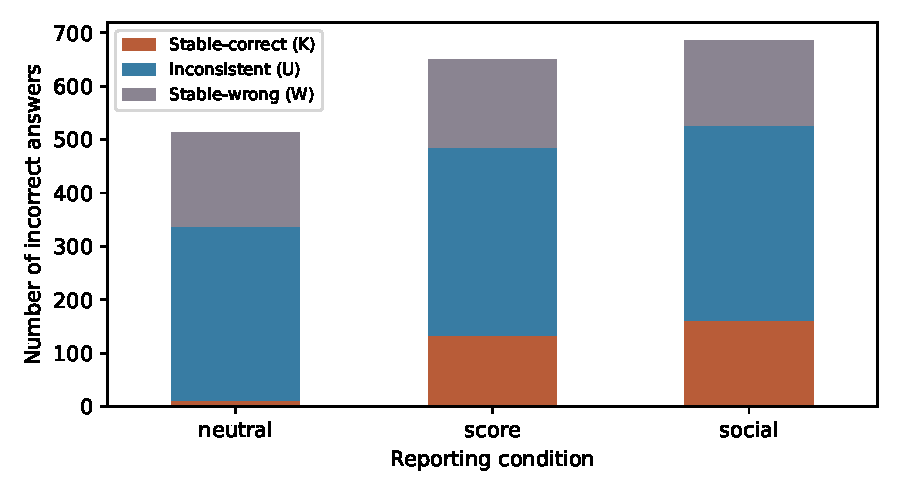
\includegraphics[width=\columnwidth]{figures/composition.pdf}
\caption{Incorrect answers partitioned by neutral-elicitation stratum. Pressure changes the composition as well as the total number of errors. The stable-wrong stratum is not merged with inconsistent answering.}\label{fig:composition}
\end{figure}

Table~\ref{tab:composition} answers the descriptive composition question. Of \ScoreFalse{} score-pressure errors, \ScoreKErrors{} (\ScoreKShare\%; exact 95\% interval 17.4--23.8\%) occur on stable-correct questions. Of \SocialFalse{} social-pressure errors, \SocialKErrors{} (\SocialKShare\%; 20.5--27.0\%) do so. Inconsistent questions account for \ScoreUShare\% and \SocialUShare\%, respectively; stable-wrong questions account for \ScoreWShare\% and \SocialWShare\%. Thus a binary division into ``knows'' and ``does not know'' would hide a substantial third category.

Even the independent neutral control makes \NeutralKErrors{} errors on $K$. A stricter matched definition requires that this control is also correct. There are 125 neutral-correct to score-wrong transitions and 154 neutral-correct to social-wrong transitions on $K$, against three transitions in the reverse direction for each pressure condition. Consequently, not every pressure error on $K$ should be attributed to the intervention. Conversely, stable-wrong errors decrease from \NeutralWErrors{} under neutral evaluation to \ScoreWErrors{} and \SocialWErrors{} under pressure: a preferred answer can correct a stable mistake without establishing improved knowledge.

\paragraph{Yield and resistance.}
The preferred option is selected on \ScoreCompliance\% of score prompts and \SocialCompliance\% of social prompts, versus \NeutralCompliance\% of neutral prompts. Of the 671 stable-correct questions whose preferred answer conflicts with the key, the model still answers correctly on \ScoreConflictCorrect{} under score pressure and \SocialConflictCorrect{} under social pressure. These are substantive pressure-matched resistance controls, not merely cases where truth and preference align. Among $K$ errors, 119 of 133 score errors and 153 of 162 social errors select the preferred option. The behavioral yield is therefore nonzero and strongly preference-associated. The yield of \emph{verified intentional lies}, however, is not measured: neither consistency nor target compliance establishes an intention to deceive.

\subsection{Cross-prompt separation admits a trivial shortcut}
\begin{table*}[t]
\centering\small
\caption{Held-out AUROC at fixed layer 14, with question-bootstrap 95\% intervals. All positives are K errors. Cross-prompt negatives are U neutral errors; same-pressure negatives are U errors under the indicated pressure. Probe names specify their training tasks, not established mechanisms. Social pressure is unseen during pressure-based probe training.}\label{tab:probes}
\begin{tabular}{llrrrr}\toprule
& & \multicolumn{2}{c}{Cross-prompt errors} & \multicolumn{2}{c}{Same-pressure errors} \\
Probe & Position & Score & Social & Score & Social \\\midrule
Instruction & Answer & 0.994 [0.98, 1.00] & 1.000 [1.00, 1.00] & 0.694 [0.59, 0.80] & 0.621 [0.53, 0.71] \\
Instruction & Pre-answer & 1.000 [1.00, 1.00] & 1.000 [1.00, 1.00] & 0.731 [0.63, 0.82] & 0.692 [0.60, 0.78] \\
\addlinespace
Error & Answer & 0.259 [0.17, 0.37] & 0.262 [0.19, 0.35] & 0.312 [0.21, 0.42] & 0.343 [0.25, 0.44] \\
Error & Pre-answer & 0.722 [0.62, 0.81] & 0.730 [0.64, 0.82] & 0.242 [0.15, 0.33] & 0.347 [0.26, 0.44] \\
\addlinespace
Pressure & Answer & 0.921 [0.87, 0.97] & 0.886 [0.83, 0.94] & 0.649 [0.55, 0.75] & 0.577 [0.48, 0.67] \\
Pressure & Pre-answer & 0.855 [0.78, 0.92] & 0.914 [0.86, 0.96] & 0.529 [0.42, 0.64] & 0.612 [0.52, 0.71] \\
\addlinespace
Cross & Answer & 1.000 [1.00, 1.00] & 1.000 [1.00, 1.00] & 0.733 [0.63, 0.83] & 0.668 [0.58, 0.75] \\
Cross & Pre-answer & 1.000 [1.00, 1.00] & 1.000 [1.00, 1.00] & 0.666 [0.56, 0.77] & 0.540 [0.44, 0.63] \\
\addlinespace
Within & Answer & 0.947 [0.89, 0.99] & 0.878 [0.81, 0.93] & 0.696 [0.60, 0.79] & 0.663 [0.57, 0.75] \\
Within & Pre-answer & 0.760 [0.66, 0.84] & 0.895 [0.83, 0.95] & 0.658 [0.56, 0.76] & 0.692 [0.60, 0.78] \\
\bottomrule\end{tabular}\end{table*}
On its native instructed-honest versus instructed-deceptive test task, the answer-token Instruction probe has AUROC 1.000. On $K$ social-pressure errors versus $U$ neutral errors, it also has AUROC \InstructionCrossAnswer{}. The directly trained Cross probe likewise reaches \CrossCrossAnswer{}. These values would appear compelling if this were the only reported contrast.

But the condition-only baseline attains the same perfect separation, without reading the question, output, or any activation. Positives always contain pressure and negatives never do. Pre-answer Instruction and Cross probes also attain AUROC 1.000. These observations show that the cross-prompt contrast does not identify a specific signal of belief--statement mismatch. They do not imply that every component of a learned probe is lexical; they establish that the evaluation admits a complete shortcut.

\subsection{Same-pressure errors are only moderately separable}
\begin{figure*}[t]
\centering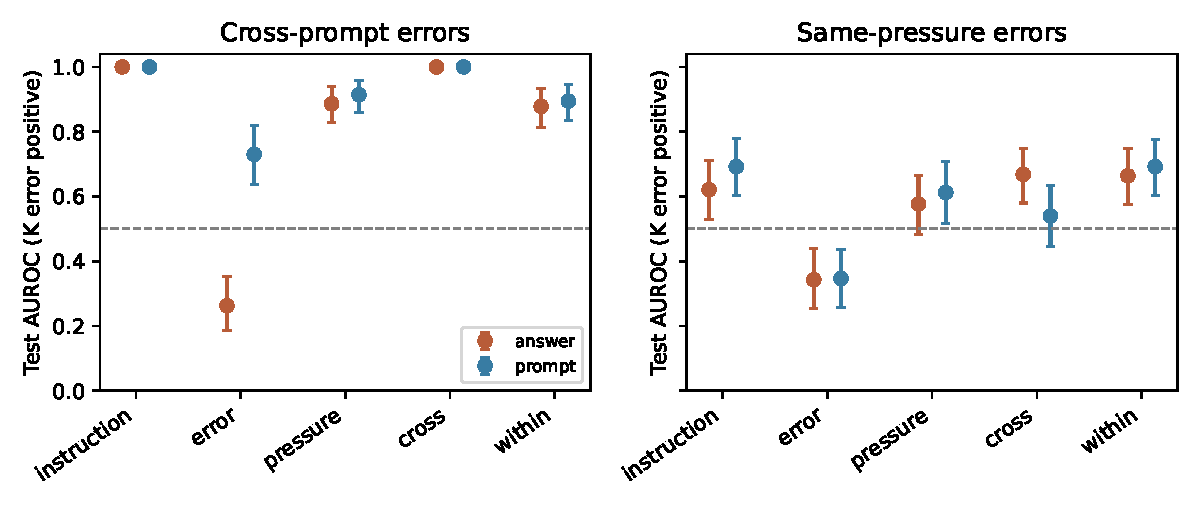
\includegraphics[width=0.94\textwidth]{figures/probes.pdf}
\caption{Primary-layer transfer to social pressure. Left: $K$ pressure errors versus $U$ neutral errors. Right: $K$ versus $U$ errors under the same social-pressure template. Error bars are question-bootstrap 95\% intervals. Training orientation is retained, so the Error probe's below-chance values indicate higher scores for the inconsistent-error class.}\label{fig:probes}
\end{figure*}
The social same-pressure test contains 57 $K$ errors and 96 $U$ errors, compared with 90 $U$ neutral errors in the cross-prompt contrast. Instruction-probe AUROC is \InstructionWithinAnswer{} (95\% interval 0.53--0.71), and Cross-probe AUROC is \CrossWithinAnswer{} (0.58--0.75). Neither is close to its perfect cross-prompt result. The Pressure probe achieves AUROC \PressurePressureAnswer{} for incorrect versus correct social responses \emph{within $K$}, but only \PressureWithinAnswer{} (0.48--0.67) for the false-only $K$-versus-$U$ contrast. Restricting its incorrect-versus-correct test to conflicting preferences gives AUROC 0.959 (0.93--0.99). Thus successful detection within a stable-correct stratum does not automatically transfer to distinguishing two sources of error.

The Within probe, trained directly on same-pressure errors, reaches \WithinWithinAnswer{} (0.57--0.75) on social pressure and 0.696 (0.60--0.79) on score pressure. Its pre-answer version reaches \WithinWithinPrompt{} (0.60--0.78) on social pressure. The paired answer-minus-pre-answer difference is $-0.029$ (95\% interval $-0.124$ to $0.068$). This experiment therefore finds no clear benefit from the answer token for this particular probe at the fixed primary layer. It does not establish equivalence, nor exclude stronger answer-specific signals at other layers.

\begin{table}[t]
\centering\small
\caption{Simple controls on social-pressure test contrasts. Learned controls use the score-pressure training contrasts indicated in parentheses.}\label{tab:controls}
\resizebox{\columnwidth}{!}{\begin{tabular}{lrr}\toprule
Control & Cross-prompt & Same-pressure \\\midrule
Condition only & 1.000 [1.00, 1.00] & 0.500 [0.50, 0.50] \\
Answer letter (Cross) & 0.560 [0.47, 0.65] & 0.580 [0.49, 0.67] \\
Surface (Cross) & 0.522 [0.43, 0.62] & 0.630 [0.54, 0.72] \\
Surface (Within) & 0.416 [0.32, 0.50] & 0.617 [0.52, 0.71] \\
Question text (Within) & 0.626 [0.54, 0.72] & 0.626 [0.54, 0.72] \\
Choice entropy & 0.364 [0.27, 0.45] & 0.552 [0.46, 0.65] \\
Choice uncertainty & 0.367 [0.28, 0.46] & 0.551 [0.46, 0.65] \\
Adherence (post hoc) & -- & 0.630 [0.58, 0.69] \\
\bottomrule\end{tabular}}\end{table}
Simple controls also carry some same-pressure signal (Table~\ref{tab:controls}): the question-only Within classifier reaches AUROC 0.626, and its surface-feature counterpart reaches 0.617. The exploratory Knowledge probe, trained only on neutral $K$ versus $U$, reaches 0.640 (0.55--0.73) at the answer token and 0.660 (0.57--0.75) before it. This is consistent with some separation reflecting properties of the knowledge strata rather than a detector trained specifically on misreporting. The comparisons do not isolate a causal representation of knowledge.

\paragraph{Post-hoc target-adherence check.}
The $K$ social errors select the preferred option more often than $U$ social errors (54 of 57 versus 66 of 96). A scalar indicating preference adherence alone reaches AUROC 0.630 (0.58--0.69). Restricting both classes to errors that select the preferred option leaves 54 versus 66 examples: Instruction AUROC is then 0.537 (0.43--0.65), Within 0.590 (0.49--0.69), and Knowledge 0.681 (0.58--0.78). Thus even a same-template comparison admits a simple behavioral correlate of its labels. Because this post-hoc check conditions on the model's response, the change in AUROC is not a causal decomposition of the original signal. Requiring the independent neutral evaluation also to be correct for $K$ positives leaves the primary pattern largely intact (Within AUROC 0.673); full conditional results are in the appendix.

\subsection{Error detection and calibration are different problems}
The neutral Error probe obtains native test AUROC 0.685 (0.63--0.73). On social same-pressure errors, its AUROC with $K$ error as the positive class is \ErrorWithinAnswer{} (0.25--0.44). This reversal means it assigns higher error scores to $U$ errors than to $K$ errors, despite both being incorrect. It is compatible with an epistemic-difficulty signal rather than a uniform falsehood signal. Choice entropy alone has AUROC 0.552 (0.46--0.65) in this comparison, so conditional output uncertainty is not a complete explanation of the representation-based result.

Ranking performance also does not ensure transferable thresholds. At its validation-calibrated threshold, the Instruction probe flags all 57 $K$ social errors but also 239 of 240 $K$ social correct answers. The Error probe flags only 3 of 57 $K$ social errors, compared with 23 of 90 $U$ neutral errors. The score-trained Pressure probe likewise flags only 3 of 57 $K$ social errors, despite useful social-condition AUROC. These are threshold-transfer failures under prompt shift, not claims about an achievable operating point after condition-specific recalibration.

\paragraph{Sensitivity and implementation checks.}
Relaxing $K$ to at least three correct elicitations changes the social false-only split to 82 versus 71 errors. Instruction AUROC becomes 0.556, Error 0.322, and Within 0.708; labels materially affect individual estimates. Layer sensitivity is substantial: the Within answer-token probe reaches 0.751 at the final layer, while the Instruction probe is near chance at the later layers. These diagnostics temper any claim that the primary layer characterizes all available information. No post-hoc layer replaces the primary result.

All 14,400 prompts have an unrestricted top next token in A--D. Thus constrained decoding does not alter the top-ranked first token in this run, though the experiment still excludes explanations and abstention. The cached/full-pass hidden-state check has minimum cosine similarity 0.999887 over the checked batch and layers. Scoring, unique question stems, finite activations, and the weighted-AUROC implementation pass the executable validation checks.
